\documentclass[twoside]{book}

% Packages required by doxygen
\usepackage{fixltx2e}
\usepackage{calc}
\usepackage{doxygen}
\usepackage[export]{adjustbox} % also loads graphicx
\usepackage{graphicx}
\usepackage[utf8]{inputenc}
\usepackage{makeidx}
\usepackage{multicol}
\usepackage{multirow}
\PassOptionsToPackage{warn}{textcomp}
\usepackage{textcomp}
\usepackage[nointegrals]{wasysym}
\usepackage[table]{xcolor}

% Font selection
\usepackage[T1]{fontenc}
\usepackage[scaled=.90]{helvet}
\usepackage{courier}
\usepackage{amssymb}
\usepackage{sectsty}
\renewcommand{\familydefault}{\sfdefault}
\allsectionsfont{%
  \fontseries{bc}\selectfont%
  \color{darkgray}%
}
\renewcommand{\DoxyLabelFont}{%
  \fontseries{bc}\selectfont%
  \color{darkgray}%
}
\newcommand{\+}{\discretionary{\mbox{\scriptsize$\hookleftarrow$}}{}{}}

% Page & text layout
\usepackage{geometry}
\geometry{%
  a4paper,%
  top=2.5cm,%
  bottom=2.5cm,%
  left=2.5cm,%
  right=2.5cm%
}
\tolerance=750
\hfuzz=15pt
\hbadness=750
\setlength{\emergencystretch}{15pt}
\setlength{\parindent}{0cm}
\setlength{\parskip}{3ex plus 2ex minus 2ex}
\makeatletter
\renewcommand{\paragraph}{%
  \@startsection{paragraph}{4}{0ex}{-1.0ex}{1.0ex}{%
    \normalfont\normalsize\bfseries\SS@parafont%
  }%
}
\renewcommand{\subparagraph}{%
  \@startsection{subparagraph}{5}{0ex}{-1.0ex}{1.0ex}{%
    \normalfont\normalsize\bfseries\SS@subparafont%
  }%
}
\makeatother

% Headers & footers
\usepackage{fancyhdr}
\pagestyle{fancyplain}
\fancyhead[LE]{\fancyplain{}{\bfseries\thepage}}
\fancyhead[CE]{\fancyplain{}{}}
\fancyhead[RE]{\fancyplain{}{\bfseries\leftmark}}
\fancyhead[LO]{\fancyplain{}{\bfseries\rightmark}}
\fancyhead[CO]{\fancyplain{}{}}
\fancyhead[RO]{\fancyplain{}{\bfseries\thepage}}
\fancyfoot[LE]{\fancyplain{}{}}
\fancyfoot[CE]{\fancyplain{}{}}
\fancyfoot[RE]{\fancyplain{}{\bfseries\scriptsize Generated by Doxygen }}
\fancyfoot[LO]{\fancyplain{}{\bfseries\scriptsize Generated by Doxygen }}
\fancyfoot[CO]{\fancyplain{}{}}
\fancyfoot[RO]{\fancyplain{}{}}
\renewcommand{\footrulewidth}{0.4pt}
\renewcommand{\chaptermark}[1]{%
  \markboth{#1}{}%
}
\renewcommand{\sectionmark}[1]{%
  \markright{\thesection\ #1}%
}

% Indices & bibliography
\usepackage{natbib}
\usepackage[titles]{tocloft}
\setcounter{tocdepth}{3}
\setcounter{secnumdepth}{5}
\makeindex

% Hyperlinks (required, but should be loaded last)
\usepackage{ifpdf}
\ifpdf
  \usepackage[pdftex,pagebackref=true]{hyperref}
\else
  \usepackage[ps2pdf,pagebackref=true]{hyperref}
\fi
\hypersetup{%
  colorlinks=true,%
  linkcolor=blue,%
  citecolor=blue,%
  unicode%
}

% Custom commands
\newcommand{\clearemptydoublepage}{%
  \newpage{\pagestyle{empty}\cleardoublepage}%
}

\usepackage{caption}
\captionsetup{labelsep=space,justification=centering,font={bf},singlelinecheck=off,skip=4pt,position=top}

%===== C O N T E N T S =====

\begin{document}

% Titlepage & ToC
\hypersetup{pageanchor=false,
             bookmarksnumbered=true,
             pdfencoding=unicode
            }
\pagenumbering{alph}
\begin{titlepage}
\vspace*{7cm}
\begin{center}%
{\Large Zu\+Car Model \\[1ex]\large 1.\+0 }\\
\vspace*{1cm}
{\large Generated by Doxygen 1.8.13}\\
\end{center}
\end{titlepage}
\clearemptydoublepage
\pagenumbering{roman}
\tableofcontents
\clearemptydoublepage
\pagenumbering{arabic}
\hypersetup{pageanchor=true}

%--- Begin generated contents ---
\chapter{Namespace Index}
\section{Namespace List}
Here is a list of all documented namespaces with brief descriptions\+:\begin{DoxyCompactList}
\item\contentsline{section}{\hyperlink{namespace_path}{Path} \\*G\+Lobal Namespace For All Car-\/like Robot Calculations }{\pageref{namespace_path}}{}
\item\contentsline{section}{\hyperlink{namespace_path_1_1_frenet_model}{Path\+::\+Frenet\+Model} \\*Namespace used to define frenet Model For Car like robots }{\pageref{namespace_path_1_1_frenet_model}}{}
\item\contentsline{section}{\hyperlink{namespace_path_1_1_kinematic_models}{Path\+::\+Kinematic\+Models} \\*Kinematic Model namespace }{\pageref{namespace_path_1_1_kinematic_models}}{}
\item\contentsline{section}{\hyperlink{namespace_path_1_1_r_control}{Path\+::\+R\+Control} \\*Namespace is describes the model of Genarlized Form of chained car like robot }{\pageref{namespace_path_1_1_r_control}}{}
\end{DoxyCompactList}

\chapter{Class Index}
\section{Class List}
Here are the classes, structs, unions and interfaces with brief descriptions\+:\begin{DoxyCompactList}
\item\contentsline{section}{\hyperlink{class_path_1_1_kinematic_models_1_1_car_description}{Path\+::\+Kinematic\+Models\+::\+Car\+Description} \\*The \hyperlink{class_path_1_1_kinematic_models_1_1_car_description}{Path\+::\+Kinematic\+Models\+::\+Car\+Description} class is used To Encapsulate Car Descriptions }{\pageref{class_path_1_1_kinematic_models_1_1_car_description}}{}
\item\contentsline{section}{\hyperlink{class_path_1_1_kinematic_models_1_1_kinematic_model}{Path\+::\+Kinematic\+Models\+::\+Kinematic\+Model} }{\pageref{class_path_1_1_kinematic_models_1_1_kinematic_model}}{}
\end{DoxyCompactList}

\chapter{Namespace Documentation}
\hypertarget{namespace_path}{}\section{Path Namespace Reference}
\label{namespace_path}\index{Path@{Path}}


G\+Lobal Namespace For All Car-\/like Robot Calculations.  


\subsection*{Namespaces}
\begin{DoxyCompactItemize}
\item 
 \hyperlink{namespace_path_1_1_frenet_model}{Frenet\+Model}
\begin{DoxyCompactList}\small\item\em namespace used to define frenet Model For Car like robots \end{DoxyCompactList}\item 
 \hyperlink{namespace_path_1_1_kinematic_models}{Kinematic\+Models}
\begin{DoxyCompactList}\small\item\em Kinematic Model namespace. \end{DoxyCompactList}\item 
 \hyperlink{namespace_path_1_1_r_control}{R\+Control}
\begin{DoxyCompactList}\small\item\em the namespace is describes the model of Genarlized Form of chained car like robot \end{DoxyCompactList}\end{DoxyCompactItemize}


\subsection{Detailed Description}
G\+Lobal Namespace For All Car-\/like Robot Calculations. 


\hypertarget{namespace_path_1_1_frenet_model}{}\section{Path\+:\+:Frenet\+Model Namespace Reference}
\label{namespace_path_1_1_frenet_model}\index{Path\+::\+Frenet\+Model@{Path\+::\+Frenet\+Model}}


namespace used to define frenet Model For Car like robots  


\subsection*{Functions}
\begin{DoxyCompactItemize}
\item 
{\footnotesize template$<$typename Num , typename Degree $>$ }\\Num \hyperlink{namespace_path_1_1_frenet_model_aad575bf8ab643cee69a04fd260537bf5}{dS} (const Num \&u1, const Num \&dc, const Degree \&theta\+\_\+e, const Degree \&phie, const Num \&lnth, const Num \&l1, const Num \&l2)
\begin{DoxyCompactList}\small\item\em this function is used to calculate differntial of S . \end{DoxyCompactList}\item 
{\footnotesize template$<$typename Num , typename Degree $>$ }\\Num \hyperlink{namespace_path_1_1_frenet_model_ad4b6f15d18cda83a0b49196c7e4c39a7}{dD} (const Num \&u1, const Degree \&theta\+\_\+e, const Degree \&phie, const Num \&lnth, const Num \&l1, const Num \&l2)
\begin{DoxyCompactList}\small\item\em this function is used to calculate differntial of d . \end{DoxyCompactList}\item 
{\footnotesize template$<$typename Num , typename Degree $>$ }\\Num \hyperlink{namespace_path_1_1_frenet_model_a353a17af4ea254880a0186a6d82a98bc}{d\+Theta} (const Num \&u1, const Num \&lnth, const Degree \&phie, const Degree \&sdot, const Degree \&c)
\begin{DoxyCompactList}\small\item\em used to calclate differntial of Theta by time \end{DoxyCompactList}\item 
{\footnotesize template$<$typename Num $>$ }\\Num \hyperlink{namespace_path_1_1_frenet_model_a5412f0a54c36b34975e06b311a411122}{d\+Phie} (const Num \&u2)
\begin{DoxyCompactList}\small\item\em used to calclate d\+Phie \end{DoxyCompactList}\end{DoxyCompactItemize}


\subsection{Detailed Description}
namespace used to define frenet Model For Car like robots 



\subsection{Function Documentation}
\mbox{\Hypertarget{namespace_path_1_1_frenet_model_ad4b6f15d18cda83a0b49196c7e4c39a7}\label{namespace_path_1_1_frenet_model_ad4b6f15d18cda83a0b49196c7e4c39a7}} 
\index{Path\+::\+Frenet\+Model@{Path\+::\+Frenet\+Model}!dD@{dD}}
\index{dD@{dD}!Path\+::\+Frenet\+Model@{Path\+::\+Frenet\+Model}}
\subsubsection{\texorpdfstring{d\+D()}{dD()}}
{\footnotesize\ttfamily template$<$typename Num , typename Degree $>$ \\
Num Path\+::\+Frenet\+Model\+::dD (\begin{DoxyParamCaption}\item[{const Num \&}]{u1,  }\item[{const Degree \&}]{theta\+\_\+e,  }\item[{const Degree \&}]{phie,  }\item[{const Num \&}]{lnth,  }\item[{const Num \&}]{l1,  }\item[{const Num \&}]{l2 }\end{DoxyParamCaption})}



this function is used to calculate differntial of d . 

the Template function uses the formula {\bfseries d˙} = u1 $\ast$ ( sin(θe) + ( (tanφ)/L) $\ast$ ( l1$\ast$cos(θe) -\/ l2$\ast$sin(θe) ) ) ) . 
\begin{DoxyParams}{Parameters}
{\em u1} & the longitudianl velocity of the robot \\
\hline
{\em lnth} & the distance between front wheels and rear wheels axle. \\
\hline
{\em phie} & The Vehicle\textquotesingle{}s steering angle. \\
\hline
{\em theta\+\_\+e} & the angle characterizing the orientation of the robot chassis with respect to the fram Fs. \\
\hline
{\em l1} & the coordinate of P (l1,l2) expressed in the basis of Fm. \\
\hline
{\em l2} & the coordinate of P (l1,l2) expressed in the basis of Fm. \\
\hline
\end{DoxyParams}
\begin{DoxyReturn}{Returns}
of Type Num the current diffrential. 
\end{DoxyReturn}
\begin{DoxyAuthor}{Author}
Sherif Abaza. 
\end{DoxyAuthor}
\mbox{\Hypertarget{namespace_path_1_1_frenet_model_a5412f0a54c36b34975e06b311a411122}\label{namespace_path_1_1_frenet_model_a5412f0a54c36b34975e06b311a411122}} 
\index{Path\+::\+Frenet\+Model@{Path\+::\+Frenet\+Model}!d\+Phie@{d\+Phie}}
\index{d\+Phie@{d\+Phie}!Path\+::\+Frenet\+Model@{Path\+::\+Frenet\+Model}}
\subsubsection{\texorpdfstring{d\+Phie()}{dPhie()}}
{\footnotesize\ttfamily template$<$typename Num $>$ \\
Num Path\+::\+Frenet\+Model\+::d\+Phie (\begin{DoxyParamCaption}\item[{const Num \&}]{u2 }\end{DoxyParamCaption})}



used to calclate d\+Phie 

the Template function uses the formula {\bfseries φ˙} = u2. 
\begin{DoxyParams}{Parameters}
{\em u2} & the angular velocity of the robot. \\
\hline
\end{DoxyParams}
\begin{DoxyReturn}{Returns}
of Type Num the current diffrential. 
\end{DoxyReturn}
\begin{DoxyAuthor}{Author}
Sherif Abaza. 
\end{DoxyAuthor}
\mbox{\Hypertarget{namespace_path_1_1_frenet_model_aad575bf8ab643cee69a04fd260537bf5}\label{namespace_path_1_1_frenet_model_aad575bf8ab643cee69a04fd260537bf5}} 
\index{Path\+::\+Frenet\+Model@{Path\+::\+Frenet\+Model}!dS@{dS}}
\index{dS@{dS}!Path\+::\+Frenet\+Model@{Path\+::\+Frenet\+Model}}
\subsubsection{\texorpdfstring{d\+S()}{dS()}}
{\footnotesize\ttfamily template$<$typename Num , typename Degree $>$ \\
Num Path\+::\+Frenet\+Model\+::dS (\begin{DoxyParamCaption}\item[{const Num \&}]{u1,  }\item[{const Num \&}]{dc,  }\item[{const Degree \&}]{theta\+\_\+e,  }\item[{const Degree \&}]{phie,  }\item[{const Num \&}]{lnth,  }\item[{const Num \&}]{l1,  }\item[{const Num \&}]{l2 }\end{DoxyParamCaption})}



this function is used to calculate differntial of S . 

the Template function uses the formula {\bfseries S˙} = ( u1 / ( 1-\/dc(s) ) ) $\ast$ ( cos(θe) -\/ ( (tanφ)/L) $\ast$ ( l2$\ast$cos(θe) + l1$\ast$sin(θe) ) ) . 
\begin{DoxyParams}{Parameters}
{\em u1} & the longitudianl velocity of the robot \\
\hline
{\em lnth} & the distance between front wheels and rear wheels axle. \\
\hline
{\em phie} & The Vehicle\textquotesingle{}s steering angle. \\
\hline
{\em theta\+\_\+e} & the angle characterizing the orientation of the robot chassis with respect to the fram Fs. \\
\hline
{\em l1} & the coordinate of P (l1,l2) expressed in the basis of Fm. \\
\hline
{\em l2} & the coordinate of P (l1,l2) expressed in the basis of Fm. \\
\hline
{\em dc} & is the differential eq of the curvature c(\+S) \\
\hline
\end{DoxyParams}
\begin{DoxyReturn}{Returns}
of Type Num the current diffrential. 
\end{DoxyReturn}
\begin{DoxyAuthor}{Author}
Sherif Abaza. 
\end{DoxyAuthor}
\mbox{\Hypertarget{namespace_path_1_1_frenet_model_a353a17af4ea254880a0186a6d82a98bc}\label{namespace_path_1_1_frenet_model_a353a17af4ea254880a0186a6d82a98bc}} 
\index{Path\+::\+Frenet\+Model@{Path\+::\+Frenet\+Model}!d\+Theta@{d\+Theta}}
\index{d\+Theta@{d\+Theta}!Path\+::\+Frenet\+Model@{Path\+::\+Frenet\+Model}}
\subsubsection{\texorpdfstring{d\+Theta()}{dTheta()}}
{\footnotesize\ttfamily template$<$typename Num , typename Degree $>$ \\
Num Path\+::\+Frenet\+Model\+::d\+Theta (\begin{DoxyParamCaption}\item[{const Num \&}]{u1,  }\item[{const Num \&}]{lnth,  }\item[{const Degree \&}]{phie,  }\item[{const Degree \&}]{sdot,  }\item[{const Degree \&}]{c }\end{DoxyParamCaption})}



used to calclate differntial of Theta by time 

the Template function uses the formula {\bfseries θ˙} = (u1/L) $\ast$ tanφ -\/ S˙\+C(\+S) . 
\begin{DoxyParams}{Parameters}
{\em u1} & the longitudianl velocity of the robot \\
\hline
{\em lnth} & the distance between front wheels and rear wheels axle. \\
\hline
{\em phie} & The Vehicle\textquotesingle{}s steering angle. \\
\hline
{\em sdot} & is the differential eqquation of the curvilinear abscissa \\
\hline
{\em c} & the curvature c(\+S) of C at Ps \\
\hline
\end{DoxyParams}
\begin{DoxyReturn}{Returns}
of Type Num the current diffrential. 
\end{DoxyReturn}
\begin{DoxyAuthor}{Author}
Sherif Abaza. 
\end{DoxyAuthor}

\hypertarget{namespace_path_1_1_kinematic_models}{}\section{Path\+:\+:Kinematic\+Models Namespace Reference}
\label{namespace_path_1_1_kinematic_models}\index{Path\+::\+Kinematic\+Models@{Path\+::\+Kinematic\+Models}}


Kinematic Model namespace.  


\subsection*{Classes}
\begin{DoxyCompactItemize}
\item 
class \hyperlink{class_path_1_1_kinematic_models_1_1_car_description}{Car\+Description}
\begin{DoxyCompactList}\small\item\em The \hyperlink{class_path_1_1_kinematic_models_1_1_car_description}{Path\+::\+Kinematic\+Models\+::\+Car\+Description} class is used To Encapsulate Car Descriptions. \end{DoxyCompactList}\item 
class \hyperlink{class_path_1_1_kinematic_models_1_1_kinematic_model}{Kinematic\+Model}
\end{DoxyCompactItemize}
\subsection*{Functions}
\begin{DoxyCompactItemize}
\item 
{\footnotesize template$<$typename Num $>$ }\\Num \hyperlink{namespace_path_1_1_kinematic_models_aaea8f9ef18514642886a2a79bb862202}{long\+Velocity} (const Num \&r, const Num \&angular\+VL, const Num \&angular\+VR)
\begin{DoxyCompactList}\small\item\em this Function is used To Cacluate Longitudinal Velocity of veichle. \end{DoxyCompactList}\item 
{\footnotesize template$<$typename Num $>$ }\\Num \hyperlink{namespace_path_1_1_kinematic_models_a340b21962938fd668f09d8cc538e3533}{rotational\+Velocity} (const Num \&r, const Num \&d\+LR, const Num \&angular\+VL, const Num \&angular\+VR)
\begin{DoxyCompactList}\small\item\em This template function used to calculate Rotational Velocity of robot. \end{DoxyCompactList}\item 
{\footnotesize template$<$typename Num , typename Degree $>$ }\\Num \hyperlink{namespace_path_1_1_kinematic_models_a552124dfc86f88feab9d659464ab2c3d}{dX} (const Num \&u1, const Degree \&theta)
\begin{DoxyCompactList}\small\item\em used to calclate diffrential of x by time \end{DoxyCompactList}\item 
{\footnotesize template$<$typename Num , typename Degree $>$ }\\Num \hyperlink{namespace_path_1_1_kinematic_models_a11aaf1219f56249da986fe9e06942d22}{dY} (const Num \&u1, const Degree \&theta)
\begin{DoxyCompactList}\small\item\em used to calclate dy \end{DoxyCompactList}\item 
{\footnotesize template$<$typename Num , typename Degree $>$ }\\Num \hyperlink{namespace_path_1_1_kinematic_models_a854b3503bce18b979159dee90ee1db0d}{d\+Theta} (const Num \&u1, const Num \&lnth, const Degree \&theta)
\begin{DoxyCompactList}\small\item\em used to calclate differntial of Theta by time \end{DoxyCompactList}\item 
{\footnotesize template$<$typename Num $>$ }\\Num \hyperlink{namespace_path_1_1_kinematic_models_a3433ae2dd28c9f7b8b66c42c173ce543}{d\+Phie} (const Num \&u2)
\begin{DoxyCompactList}\small\item\em used to calclate d\+Phie \end{DoxyCompactList}\item 
{\footnotesize template$<$typename Num $>$ }\\Num D\+E\+C\+L\+A\+R\+\_\+\+L\+IB \hyperlink{namespace_path_1_1_kinematic_models_a1d71a0052e6781a914b7734f61ccda59}{long\+Velocity} (const Num \&r, const Num \&angular\+VL, const Num \&angular\+VR)
\begin{DoxyCompactList}\small\item\em this Function is used To Cacluate Longitudinal Velocity of veichle. \end{DoxyCompactList}\item 
{\footnotesize template$<$typename Num $>$ }\\Num D\+E\+C\+L\+A\+R\+\_\+\+L\+IB \hyperlink{namespace_path_1_1_kinematic_models_a12c28f2e1b73152b0f51af632889bc4f}{rotational\+Velocity} (const Num \&r, const Num \&d\+LR, const Num \&angular\+VL, const Num \&angular\+VR)
\begin{DoxyCompactList}\small\item\em This template function used to calculate Rotational Velocity of robot. \end{DoxyCompactList}\item 
{\footnotesize template$<$typename Num , typename Degree $>$ }\\Num D\+E\+C\+L\+A\+R\+\_\+\+L\+IB \hyperlink{namespace_path_1_1_kinematic_models_a28f62881ebe7e125d5039f52b72448b5}{dX} (const Num \&u1, const Degree \&theta)
\begin{DoxyCompactList}\small\item\em used to calclate diffrential of x by time \end{DoxyCompactList}\item 
{\footnotesize template$<$typename Num , typename Degree $>$ }\\Num D\+E\+C\+L\+A\+R\+\_\+\+L\+IB \hyperlink{namespace_path_1_1_kinematic_models_a872e84d8a115db786624f3fc8e6790a4}{dY} (const Num \&u1, const Degree \&theta)
\begin{DoxyCompactList}\small\item\em used to calclate dy \end{DoxyCompactList}\item 
{\footnotesize template$<$typename Num , typename Degree $>$ }\\Num D\+E\+C\+L\+A\+R\+\_\+\+L\+IB \hyperlink{namespace_path_1_1_kinematic_models_ae5c91053b1ebb8437864fcd208a45d27}{d\+Theta} (const Num \&u1, const Num \&lnth, const Degree \&theta)
\begin{DoxyCompactList}\small\item\em used to calclate differntial of Theta by time \end{DoxyCompactList}\item 
{\footnotesize template$<$typename Num $>$ }\\Num D\+E\+C\+L\+A\+R\+\_\+\+L\+IB \hyperlink{namespace_path_1_1_kinematic_models_a9056e401aa320699847d4ab3b3e73a98}{d\+Phie} (const Num \&u2)
\begin{DoxyCompactList}\small\item\em used to calclate d\+Phie \end{DoxyCompactList}\end{DoxyCompactItemize}
\subsection*{Variables}
\begin{DoxyCompactItemize}
\item 
\mbox{\Hypertarget{namespace_path_1_1_kinematic_models_a3c42bccfe7cadc3cdc95b21d247ba71d}\label{namespace_path_1_1_kinematic_models_a3c42bccfe7cadc3cdc95b21d247ba71d}} 
class D\+E\+C\+L\+A\+R\+\_\+\+L\+IB {\bfseries Kinematic\+Model}
\item 
\mbox{\Hypertarget{namespace_path_1_1_kinematic_models_a963c2abaa9c22129daad361ab3c4183e}\label{namespace_path_1_1_kinematic_models_a963c2abaa9c22129daad361ab3c4183e}} 
class D\+E\+C\+L\+A\+R\+\_\+\+L\+IB {\bfseries Car\+Description}
\end{DoxyCompactItemize}


\subsection{Detailed Description}
Kinematic Model namespace. 

\begin{DoxyAuthor}{Author}
Mohamed Khaled.
\end{DoxyAuthor}
This Namespace Describes The Basic General Kinematic functions for car like {\bfseries robots}.  \begin{DoxyParagraph}{uses the equations}
{\bfseries  x˙ = u1 cosθ , ~\newline
 y˙ = u1 sinθ , ~\newline
 θ˙ = (u1/L) $\ast$ tanφ , ~\newline
 φ˙ = u2 , ~\newline
 } 
\end{DoxyParagraph}


\subsection{Function Documentation}
\mbox{\Hypertarget{namespace_path_1_1_kinematic_models_a9056e401aa320699847d4ab3b3e73a98}\label{namespace_path_1_1_kinematic_models_a9056e401aa320699847d4ab3b3e73a98}} 
\index{Path\+::\+Kinematic\+Models@{Path\+::\+Kinematic\+Models}!d\+Phie@{d\+Phie}}
\index{d\+Phie@{d\+Phie}!Path\+::\+Kinematic\+Models@{Path\+::\+Kinematic\+Models}}
\subsubsection{\texorpdfstring{d\+Phie()}{dPhie()}\hspace{0.1cm}{\footnotesize\ttfamily [1/2]}}
{\footnotesize\ttfamily template$<$typename Num $>$ \\
Num D\+E\+C\+L\+A\+R\+\_\+\+L\+IB Path\+::\+Kinematic\+Models\+::d\+Phie (\begin{DoxyParamCaption}\item[{const Num \&}]{u2 }\end{DoxyParamCaption})}



used to calclate d\+Phie 

the Template function uses the formula {\bfseries φ˙} = u2. 
\begin{DoxyParams}{Parameters}
{\em u2} & the angular velocity of the robot. \\
\hline
\end{DoxyParams}
\begin{DoxyReturn}{Returns}
of Type Num the current diffrential. 
\end{DoxyReturn}
\begin{DoxyAuthor}{Author}
Mohamed Khaled.
\end{DoxyAuthor}
the Template function uses the formula {\bfseries φ˙} = u2. 
\begin{DoxyParams}{Parameters}
{\em u2} & the angular velocity of the robot. \\
\hline
\end{DoxyParams}
\begin{DoxyReturn}{Returns}
of Type Num the current diffrential. 
\end{DoxyReturn}
\begin{DoxyAuthor}{Author}
Sherif Abaza. 
\end{DoxyAuthor}
\mbox{\Hypertarget{namespace_path_1_1_kinematic_models_a3433ae2dd28c9f7b8b66c42c173ce543}\label{namespace_path_1_1_kinematic_models_a3433ae2dd28c9f7b8b66c42c173ce543}} 
\index{Path\+::\+Kinematic\+Models@{Path\+::\+Kinematic\+Models}!d\+Phie@{d\+Phie}}
\index{d\+Phie@{d\+Phie}!Path\+::\+Kinematic\+Models@{Path\+::\+Kinematic\+Models}}
\subsubsection{\texorpdfstring{d\+Phie()}{dPhie()}\hspace{0.1cm}{\footnotesize\ttfamily [2/2]}}
{\footnotesize\ttfamily template$<$typename Num $>$ \\
Num Path\+::\+Kinematic\+Models\+::d\+Phie (\begin{DoxyParamCaption}\item[{const Num \&}]{u2 }\end{DoxyParamCaption})}



used to calclate d\+Phie 

the Template function uses the formula {\bfseries φ˙} = u2. 
\begin{DoxyParams}{Parameters}
{\em u2} & the angular velocity of the robot. \\
\hline
\end{DoxyParams}
\begin{DoxyReturn}{Returns}
of Type Num the current diffrential. 
\end{DoxyReturn}
\begin{DoxyAuthor}{Author}
Mohamed Khaled. 
\end{DoxyAuthor}
\mbox{\Hypertarget{namespace_path_1_1_kinematic_models_ae5c91053b1ebb8437864fcd208a45d27}\label{namespace_path_1_1_kinematic_models_ae5c91053b1ebb8437864fcd208a45d27}} 
\index{Path\+::\+Kinematic\+Models@{Path\+::\+Kinematic\+Models}!d\+Theta@{d\+Theta}}
\index{d\+Theta@{d\+Theta}!Path\+::\+Kinematic\+Models@{Path\+::\+Kinematic\+Models}}
\subsubsection{\texorpdfstring{d\+Theta()}{dTheta()}\hspace{0.1cm}{\footnotesize\ttfamily [1/2]}}
{\footnotesize\ttfamily template$<$typename Num , typename Degree $>$ \\
Num D\+E\+C\+L\+A\+R\+\_\+\+L\+IB Path\+::\+Kinematic\+Models\+::d\+Theta (\begin{DoxyParamCaption}\item[{const Num \&}]{u1,  }\item[{const Num \&}]{lnth,  }\item[{const Degree \&}]{theta }\end{DoxyParamCaption})}



used to calclate differntial of Theta by time 

the Template function uses the formula {\bfseries θ˙} = (u1/L) $\ast$ tanφ . 
\begin{DoxyParams}{Parameters}
{\em u1} & the longitudianl velocity of the robot \\
\hline
{\em lngth} & the distance between front wheels and rear wheels axle. \\
\hline
{\em theta} & the angle of the robot chassis orientation . \\
\hline
\end{DoxyParams}
\begin{DoxyReturn}{Returns}
of Type Num the current diffrential. 
\end{DoxyReturn}
\begin{DoxyAuthor}{Author}
Mohamed Khaled. 
\end{DoxyAuthor}
\mbox{\Hypertarget{namespace_path_1_1_kinematic_models_a854b3503bce18b979159dee90ee1db0d}\label{namespace_path_1_1_kinematic_models_a854b3503bce18b979159dee90ee1db0d}} 
\index{Path\+::\+Kinematic\+Models@{Path\+::\+Kinematic\+Models}!d\+Theta@{d\+Theta}}
\index{d\+Theta@{d\+Theta}!Path\+::\+Kinematic\+Models@{Path\+::\+Kinematic\+Models}}
\subsubsection{\texorpdfstring{d\+Theta()}{dTheta()}\hspace{0.1cm}{\footnotesize\ttfamily [2/2]}}
{\footnotesize\ttfamily template$<$typename Num , typename Degree $>$ \\
Num Path\+::\+Kinematic\+Models\+::d\+Theta (\begin{DoxyParamCaption}\item[{const Num \&}]{u1,  }\item[{const Num \&}]{lnth,  }\item[{const Degree \&}]{theta }\end{DoxyParamCaption})}



used to calclate differntial of Theta by time 

the Template function uses the formula {\bfseries θ˙} = (u1/L) $\ast$ tanφ . 
\begin{DoxyParams}{Parameters}
{\em u1} & the longitudianl velocity of the robot \\
\hline
{\em lngth} & the distance between front wheels and rear wheels axle. \\
\hline
{\em theta} & the angle of the robot chassis orientation . \\
\hline
\end{DoxyParams}
\begin{DoxyReturn}{Returns}
of Type Num the current diffrential. 
\end{DoxyReturn}
\begin{DoxyAuthor}{Author}
Mohamed Khaled. 
\end{DoxyAuthor}
\mbox{\Hypertarget{namespace_path_1_1_kinematic_models_a28f62881ebe7e125d5039f52b72448b5}\label{namespace_path_1_1_kinematic_models_a28f62881ebe7e125d5039f52b72448b5}} 
\index{Path\+::\+Kinematic\+Models@{Path\+::\+Kinematic\+Models}!dX@{dX}}
\index{dX@{dX}!Path\+::\+Kinematic\+Models@{Path\+::\+Kinematic\+Models}}
\subsubsection{\texorpdfstring{d\+X()}{dX()}\hspace{0.1cm}{\footnotesize\ttfamily [1/2]}}
{\footnotesize\ttfamily template$<$typename Num , typename Degree $>$ \\
Num D\+E\+C\+L\+A\+R\+\_\+\+L\+IB Path\+::\+Kinematic\+Models\+::dX (\begin{DoxyParamCaption}\item[{const Num \&}]{u1,  }\item[{const Degree \&}]{theta }\end{DoxyParamCaption})}



used to calclate diffrential of x by time 

the Template function uses the formula {\bfseries x˙} = u1 cosθ. 
\begin{DoxyParams}{Parameters}
{\em u1} & the longitudinal velocity of the robot \\
\hline
{\em theta} & the angle of the robot chassis orientation . \\
\hline
\end{DoxyParams}
\begin{DoxyReturn}{Returns}
of Type Num the current diffrential. 
\end{DoxyReturn}
\begin{DoxyAuthor}{Author}
Mohamed Khaled. 
\end{DoxyAuthor}
\mbox{\Hypertarget{namespace_path_1_1_kinematic_models_a552124dfc86f88feab9d659464ab2c3d}\label{namespace_path_1_1_kinematic_models_a552124dfc86f88feab9d659464ab2c3d}} 
\index{Path\+::\+Kinematic\+Models@{Path\+::\+Kinematic\+Models}!dX@{dX}}
\index{dX@{dX}!Path\+::\+Kinematic\+Models@{Path\+::\+Kinematic\+Models}}
\subsubsection{\texorpdfstring{d\+X()}{dX()}\hspace{0.1cm}{\footnotesize\ttfamily [2/2]}}
{\footnotesize\ttfamily template$<$typename Num , typename Degree $>$ \\
Num Path\+::\+Kinematic\+Models\+::dX (\begin{DoxyParamCaption}\item[{const Num \&}]{u1,  }\item[{const Degree \&}]{theta }\end{DoxyParamCaption})}



used to calclate diffrential of x by time 

the Template function uses the formula {\bfseries x˙} = u1 cosθ. 
\begin{DoxyParams}{Parameters}
{\em u1} & the longitudinal velocity of the robot \\
\hline
{\em theta} & the angle of the robot chassis orientation . \\
\hline
\end{DoxyParams}
\begin{DoxyReturn}{Returns}
of Type Num the current diffrential. 
\end{DoxyReturn}
\begin{DoxyAuthor}{Author}
Mohamed Khaled. 
\end{DoxyAuthor}
\mbox{\Hypertarget{namespace_path_1_1_kinematic_models_a872e84d8a115db786624f3fc8e6790a4}\label{namespace_path_1_1_kinematic_models_a872e84d8a115db786624f3fc8e6790a4}} 
\index{Path\+::\+Kinematic\+Models@{Path\+::\+Kinematic\+Models}!dY@{dY}}
\index{dY@{dY}!Path\+::\+Kinematic\+Models@{Path\+::\+Kinematic\+Models}}
\subsubsection{\texorpdfstring{d\+Y()}{dY()}\hspace{0.1cm}{\footnotesize\ttfamily [1/2]}}
{\footnotesize\ttfamily template$<$typename Num , typename Degree $>$ \\
Num D\+E\+C\+L\+A\+R\+\_\+\+L\+IB Path\+::\+Kinematic\+Models\+::dY (\begin{DoxyParamCaption}\item[{const Num \&}]{u1,  }\item[{const Degree \&}]{theta }\end{DoxyParamCaption})}



used to calclate dy 

the Template function uses the formula {\bfseries y˙} = u1 sinθ. 
\begin{DoxyParams}{Parameters}
{\em theta} & the angle of the robot chassis orientation . \\
\hline
\end{DoxyParams}
\begin{DoxyReturn}{Returns}
of Type Num the current diffrential. 
\end{DoxyReturn}
\begin{DoxyAuthor}{Author}
Mohamed Khaled. 
\end{DoxyAuthor}
\mbox{\Hypertarget{namespace_path_1_1_kinematic_models_a11aaf1219f56249da986fe9e06942d22}\label{namespace_path_1_1_kinematic_models_a11aaf1219f56249da986fe9e06942d22}} 
\index{Path\+::\+Kinematic\+Models@{Path\+::\+Kinematic\+Models}!dY@{dY}}
\index{dY@{dY}!Path\+::\+Kinematic\+Models@{Path\+::\+Kinematic\+Models}}
\subsubsection{\texorpdfstring{d\+Y()}{dY()}\hspace{0.1cm}{\footnotesize\ttfamily [2/2]}}
{\footnotesize\ttfamily template$<$typename Num , typename Degree $>$ \\
Num Path\+::\+Kinematic\+Models\+::dY (\begin{DoxyParamCaption}\item[{const Num \&}]{u1,  }\item[{const Degree \&}]{theta }\end{DoxyParamCaption})}



used to calclate dy 

the Template function uses the formula {\bfseries y˙} = u1 sinθ. 
\begin{DoxyParams}{Parameters}
{\em theta} & the angle of the robot chassis orientation . \\
\hline
\end{DoxyParams}
\begin{DoxyReturn}{Returns}
of Type Num the current diffrential. 
\end{DoxyReturn}
\begin{DoxyAuthor}{Author}
Mohamed Khaled. 
\end{DoxyAuthor}
\mbox{\Hypertarget{namespace_path_1_1_kinematic_models_a1d71a0052e6781a914b7734f61ccda59}\label{namespace_path_1_1_kinematic_models_a1d71a0052e6781a914b7734f61ccda59}} 
\index{Path\+::\+Kinematic\+Models@{Path\+::\+Kinematic\+Models}!long\+Velocity@{long\+Velocity}}
\index{long\+Velocity@{long\+Velocity}!Path\+::\+Kinematic\+Models@{Path\+::\+Kinematic\+Models}}
\subsubsection{\texorpdfstring{long\+Velocity()}{longVelocity()}\hspace{0.1cm}{\footnotesize\ttfamily [1/2]}}
{\footnotesize\ttfamily template$<$typename Num $>$ \\
Num D\+E\+C\+L\+A\+R\+\_\+\+L\+IB Path\+::\+Kinematic\+Models\+::long\+Velocity (\begin{DoxyParamCaption}\item[{const Num \&}]{r,  }\item[{const Num \&}]{angular\+VL,  }\item[{const Num \&}]{angular\+VR }\end{DoxyParamCaption})}



this Function is used To Cacluate Longitudinal Velocity of veichle. 

This Is a template function used to calculate the longitudinal Velocity of Robot according to the relation 
\begin{DoxyParams}{Parameters}
{\em Num} & describes The Type of return and other parameters \\
\hline
{\em r} & describes The radius of wheeles used in the car. \\
\hline
{\em angular\+VL} & angular velocity of left Wheel. \\
\hline
{\em angular\+VR} & angular velocity of right Wheel. \\
\hline
\end{DoxyParams}
\begin{DoxyReturn}{Returns}
the Longtiudnal of car Velocity. 
\end{DoxyReturn}
\begin{DoxyAuthor}{Author}
Mohamed Khaled. 
\end{DoxyAuthor}
\mbox{\Hypertarget{namespace_path_1_1_kinematic_models_aaea8f9ef18514642886a2a79bb862202}\label{namespace_path_1_1_kinematic_models_aaea8f9ef18514642886a2a79bb862202}} 
\index{Path\+::\+Kinematic\+Models@{Path\+::\+Kinematic\+Models}!long\+Velocity@{long\+Velocity}}
\index{long\+Velocity@{long\+Velocity}!Path\+::\+Kinematic\+Models@{Path\+::\+Kinematic\+Models}}
\subsubsection{\texorpdfstring{long\+Velocity()}{longVelocity()}\hspace{0.1cm}{\footnotesize\ttfamily [2/2]}}
{\footnotesize\ttfamily template$<$typename Num $>$ \\
Num Path\+::\+Kinematic\+Models\+::long\+Velocity (\begin{DoxyParamCaption}\item[{const Num \&}]{r,  }\item[{const Num \&}]{angular\+VL,  }\item[{const Num \&}]{angular\+VR }\end{DoxyParamCaption})}



this Function is used To Cacluate Longitudinal Velocity of veichle. 

This Is a template function used to calculate the longitudinal Velocity of Robot according to the relation 
\begin{DoxyParams}{Parameters}
{\em Num} & describes The Type of return and other parameters \\
\hline
{\em r} & describes The radius of wheeles used in the car. \\
\hline
{\em angular\+VL} & angular velocity of left Wheel. \\
\hline
{\em angular\+VR} & angular velocity of right Wheel. \\
\hline
\end{DoxyParams}
\begin{DoxyReturn}{Returns}
the Longtiudnal of car Velocity. 
\end{DoxyReturn}
\begin{DoxyAuthor}{Author}
Mohamed Khaled. 
\end{DoxyAuthor}
\mbox{\Hypertarget{namespace_path_1_1_kinematic_models_a12c28f2e1b73152b0f51af632889bc4f}\label{namespace_path_1_1_kinematic_models_a12c28f2e1b73152b0f51af632889bc4f}} 
\index{Path\+::\+Kinematic\+Models@{Path\+::\+Kinematic\+Models}!rotational\+Velocity@{rotational\+Velocity}}
\index{rotational\+Velocity@{rotational\+Velocity}!Path\+::\+Kinematic\+Models@{Path\+::\+Kinematic\+Models}}
\subsubsection{\texorpdfstring{rotational\+Velocity()}{rotationalVelocity()}\hspace{0.1cm}{\footnotesize\ttfamily [1/2]}}
{\footnotesize\ttfamily template$<$typename Num $>$ \\
Num D\+E\+C\+L\+A\+R\+\_\+\+L\+IB Path\+::\+Kinematic\+Models\+::rotational\+Velocity (\begin{DoxyParamCaption}\item[{const Num \&}]{r,  }\item[{const Num \&}]{d\+LR,  }\item[{const Num \&}]{angular\+VL,  }\item[{const Num \&}]{angular\+VR }\end{DoxyParamCaption})}



This template function used to calculate Rotational Velocity of robot. 

the function uses the formula {\bfseries u2} =r/2R $\ast$ (ψ˙r −ψ˙l). 
\begin{DoxyParams}{Parameters}
{\em r} & describes the radius of the wheel. \\
\hline
{\em d\+LR} & describes the distance between the left and right wheels \\
\hline
{\em angular\+VL} & angular velocity of left Wheel. \\
\hline
{\em angular\+VR} & angular velocity of right Wheel. \\
\hline
\end{DoxyParams}
\begin{DoxyReturn}{Returns}
the Velocity of rotation. 
\end{DoxyReturn}
\begin{DoxyAuthor}{Author}
Mohamed Khaled. 
\end{DoxyAuthor}
\mbox{\Hypertarget{namespace_path_1_1_kinematic_models_a340b21962938fd668f09d8cc538e3533}\label{namespace_path_1_1_kinematic_models_a340b21962938fd668f09d8cc538e3533}} 
\index{Path\+::\+Kinematic\+Models@{Path\+::\+Kinematic\+Models}!rotational\+Velocity@{rotational\+Velocity}}
\index{rotational\+Velocity@{rotational\+Velocity}!Path\+::\+Kinematic\+Models@{Path\+::\+Kinematic\+Models}}
\subsubsection{\texorpdfstring{rotational\+Velocity()}{rotationalVelocity()}\hspace{0.1cm}{\footnotesize\ttfamily [2/2]}}
{\footnotesize\ttfamily template$<$typename Num $>$ \\
Num Path\+::\+Kinematic\+Models\+::rotational\+Velocity (\begin{DoxyParamCaption}\item[{const Num \&}]{r,  }\item[{const Num \&}]{d\+LR,  }\item[{const Num \&}]{angular\+VL,  }\item[{const Num \&}]{angular\+VR }\end{DoxyParamCaption})}



This template function used to calculate Rotational Velocity of robot. 

the function uses the formula {\bfseries u2} =r/2R $\ast$ (ψ˙r −ψ˙l). 
\begin{DoxyParams}{Parameters}
{\em r} & describes the radius of the wheel. \\
\hline
{\em d\+LR} & describes the distance between the left and right wheels \\
\hline
{\em angular\+VL} & angular velocity of left Wheel. \\
\hline
{\em angular\+VR} & angular velocity of right Wheel. \\
\hline
\end{DoxyParams}
\begin{DoxyReturn}{Returns}
the Velocity of rotation. 
\end{DoxyReturn}
\begin{DoxyAuthor}{Author}
Mohamed Khaled. 
\end{DoxyAuthor}

\hypertarget{namespace_path_1_1_r_control}{}\section{Path\+:\+:R\+Control Namespace Reference}
\label{namespace_path_1_1_r_control}\index{Path\+::\+R\+Control@{Path\+::\+R\+Control}}


the namespace is describes the model of Genarlized Form of chained car like robot  


\subsection*{Functions}
\begin{DoxyCompactItemize}
\item 
\mbox{\Hypertarget{namespace_path_1_1_r_control_aed1a8a2610768324f64c8885e74b31ea}\label{namespace_path_1_1_r_control_aed1a8a2610768324f64c8885e74b31ea}} 
{\footnotesize template$<$typename Num $>$ }\\Num D\+E\+C\+L\+A\+R\+\_\+\+L\+IB {\bfseries calc\+Z1} (const Num \&s)
\item 
\mbox{\Hypertarget{namespace_path_1_1_r_control_a9c5d3dbe8dcff3ec69f468bd3a14f25e}\label{namespace_path_1_1_r_control_a9c5d3dbe8dcff3ec69f468bd3a14f25e}} 
{\footnotesize template$<$typename Num $>$ }\\Num D\+E\+C\+L\+A\+R\+\_\+\+L\+IB {\bfseries calc\+Z2} (const Num \&d)
\item 
\mbox{\Hypertarget{namespace_path_1_1_r_control_ae42a9cd1193fe31694dc236f27b265c1}\label{namespace_path_1_1_r_control_ae42a9cd1193fe31694dc236f27b265c1}} 
{\footnotesize template$<$typename Num $>$ }\\Num D\+E\+C\+L\+A\+R\+\_\+\+L\+IB {\bfseries calc\+Z3} (const Num \&d, const Num \&s, const Num \&thetaE)
\item 
\mbox{\Hypertarget{namespace_path_1_1_r_control_aced4f7869f79063e2a7f0a4fc27795d0}\label{namespace_path_1_1_r_control_aced4f7869f79063e2a7f0a4fc27795d0}} 
{\footnotesize template$<$typename Num $>$ }\\Num D\+E\+C\+L\+A\+R\+\_\+\+L\+IB {\bfseries calc\+Z4} (const Num \&d, const Num \&s, const Num \&thetaE, const Num \&phi, const Num \&L, const Num \&curvature, const Num \&curvature\+DF)
\item 
\mbox{\Hypertarget{namespace_path_1_1_r_control_a2481f54f10def70ea47eaa513e26275c}\label{namespace_path_1_1_r_control_a2481f54f10def70ea47eaa513e26275c}} 
{\footnotesize template$<$typename Num $>$ }\\Num D\+E\+C\+L\+A\+R\+\_\+\+L\+IB {\bfseries control\+Signal\+\_\+\+V2} (const Num \&v1, const Num \&k2, const Num \&k3, const Num \&K4, const Num \&k4, const Num \&z2, const Num \&z3, const Num \&z4)
\item 
\mbox{\Hypertarget{namespace_path_1_1_r_control_ad9e2cb67c7695a6c57c48e0b272eea5b}\label{namespace_path_1_1_r_control_ad9e2cb67c7695a6c57c48e0b272eea5b}} 
{\footnotesize template$<$typename Num $>$ }\\Num D\+E\+C\+L\+A\+R\+\_\+\+L\+IB {\bfseries calc\+V1} (const Num \&u1, const Num \&curvature, const Num \&d, const Num \&thetaE)
\item 
\mbox{\Hypertarget{namespace_path_1_1_r_control_a90c8fb9a17cb0e427aa59817b501e6bc}\label{namespace_path_1_1_r_control_a90c8fb9a17cb0e427aa59817b501e6bc}} 
{\footnotesize template$<$typename Num $>$ }\\Num {\bfseries calc\+Z1} (const Num \&s)
\item 
\mbox{\Hypertarget{namespace_path_1_1_r_control_adec01dfbe0a25b231d4c1d54a1989b1f}\label{namespace_path_1_1_r_control_adec01dfbe0a25b231d4c1d54a1989b1f}} 
{\footnotesize template$<$typename Num $>$ }\\Num {\bfseries calc\+Z2} (const Num \&d)
\item 
\mbox{\Hypertarget{namespace_path_1_1_r_control_a039ab9e3f03f77274b4547d2f430eeb1}\label{namespace_path_1_1_r_control_a039ab9e3f03f77274b4547d2f430eeb1}} 
{\footnotesize template$<$typename Num $>$ }\\Num {\bfseries calc\+Z3} (const Num \&d, const Num \&s, const Num \&thetaE, const Num \&curvature)
\item 
\mbox{\Hypertarget{namespace_path_1_1_r_control_aaf4ae8618fb2545cf50a7d97dadea831}\label{namespace_path_1_1_r_control_aaf4ae8618fb2545cf50a7d97dadea831}} 
{\footnotesize template$<$typename Num $>$ }\\Num {\bfseries clac\+Z4} (const Num \&d, const Num \&s, const Num \&thetaE, const Num \&phi, const Num \&L, const Num \&curvature, const Num \&curvature\+DF)
\item 
\mbox{\Hypertarget{namespace_path_1_1_r_control_a21b616a625b29729da47a39137ec1b65}\label{namespace_path_1_1_r_control_a21b616a625b29729da47a39137ec1b65}} 
{\footnotesize template$<$typename Num $>$ }\\Num {\bfseries control\+Signal\+\_\+\+V2} (const Num \&v1, const Num \&k2, const Num \&k3, const Num \&k4, const Num \&z2, const Num \&z3, const Num \&z4)
\item 
\mbox{\Hypertarget{namespace_path_1_1_r_control_a0ab88e6eaa7684d5c381effb50160261}\label{namespace_path_1_1_r_control_a0ab88e6eaa7684d5c381effb50160261}} 
{\footnotesize template$<$typename Num $>$ }\\Num {\bfseries calc\+V1} (const Num \&u1, const Num \&curvature, const Num \&d, const Num \&thetaE)
\end{DoxyCompactItemize}


\subsection{Detailed Description}
the namespace is describes the model of Genarlized Form of chained car like robot 


\chapter{Class Documentation}
\hypertarget{class_path_1_1_kinematic_models_1_1_car_description}{}\section{Path\+:\+:Kinematic\+Models\+:\+:Car\+Description Class Reference}
\label{class_path_1_1_kinematic_models_1_1_car_description}\index{Path\+::\+Kinematic\+Models\+::\+Car\+Description@{Path\+::\+Kinematic\+Models\+::\+Car\+Description}}


The \hyperlink{class_path_1_1_kinematic_models_1_1_car_description}{Path\+::\+Kinematic\+Models\+::\+Car\+Description} class is used To Encapsulate Car Descriptions.  




{\ttfamily \#include $<$cardescription.\+h$>$}



Collaboration diagram for Path\+:\+:Kinematic\+Models\+:\+:Car\+Description\+:\nopagebreak
\begin{figure}[H]
\begin{center}
\leavevmode
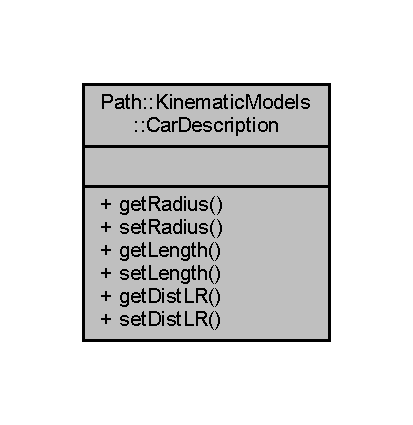
\includegraphics[width=198pt]{de/df9/class_path_1_1_kinematic_models_1_1_car_description__coll__graph}
\end{center}
\end{figure}
\subsection*{Public Member Functions}
\begin{DoxyCompactItemize}
\item 
\mbox{\Hypertarget{class_path_1_1_kinematic_models_1_1_car_description_a0a5d52772eecc8600982aa714bcd7a54}\label{class_path_1_1_kinematic_models_1_1_car_description_a0a5d52772eecc8600982aa714bcd7a54}} 
double {\bfseries get\+Radius} () const
\item 
\mbox{\Hypertarget{class_path_1_1_kinematic_models_1_1_car_description_af1610f36ec77c4c6afe36a7650f09af2}\label{class_path_1_1_kinematic_models_1_1_car_description_af1610f36ec77c4c6afe36a7650f09af2}} 
void {\bfseries set\+Radius} (double value)
\item 
\mbox{\Hypertarget{class_path_1_1_kinematic_models_1_1_car_description_a2fa8b576e5b09a039400f1ae55f01aa0}\label{class_path_1_1_kinematic_models_1_1_car_description_a2fa8b576e5b09a039400f1ae55f01aa0}} 
double {\bfseries get\+Length} () const
\item 
\mbox{\Hypertarget{class_path_1_1_kinematic_models_1_1_car_description_a61a94b23f65cb9b00c1520a951aee9a0}\label{class_path_1_1_kinematic_models_1_1_car_description_a61a94b23f65cb9b00c1520a951aee9a0}} 
void {\bfseries set\+Length} (double value)
\item 
\mbox{\Hypertarget{class_path_1_1_kinematic_models_1_1_car_description_a9626410707fb0bf0b509503d6db6730f}\label{class_path_1_1_kinematic_models_1_1_car_description_a9626410707fb0bf0b509503d6db6730f}} 
double {\bfseries get\+Dist\+LR} () const
\item 
\mbox{\Hypertarget{class_path_1_1_kinematic_models_1_1_car_description_a1a492ddd36a0be207aa408c0ec55f04d}\label{class_path_1_1_kinematic_models_1_1_car_description_a1a492ddd36a0be207aa408c0ec55f04d}} 
void {\bfseries set\+Dist\+LR} (double value)
\end{DoxyCompactItemize}


\subsection{Detailed Description}
The \hyperlink{class_path_1_1_kinematic_models_1_1_car_description}{Path\+::\+Kinematic\+Models\+::\+Car\+Description} class is used To Encapsulate Car Descriptions. 

The documentation for this class was generated from the following files\+:\begin{DoxyCompactItemize}
\item 
Car\+Model/\+Car\+Model\+Qt/\+Car\+Math\+Model/\+Path\+Tracking/cardescription.\+h\item 
Car\+Model/\+Car\+Model\+Qt/\+Car\+Math\+Model/\+Path\+Tracking/cardescription.\+cpp\end{DoxyCompactItemize}

\hypertarget{class_path_1_1_kinematic_models_1_1_kinematic_model}{}\section{Path\+:\+:Kinematic\+Models\+:\+:Kinematic\+Model Class Reference}
\label{class_path_1_1_kinematic_models_1_1_kinematic_model}\index{Path\+::\+Kinematic\+Models\+::\+Kinematic\+Model@{Path\+::\+Kinematic\+Models\+::\+Kinematic\+Model}}


Collaboration diagram for Path\+:\+:Kinematic\+Models\+:\+:Kinematic\+Model\+:\nopagebreak
\begin{figure}[H]
\begin{center}
\leavevmode
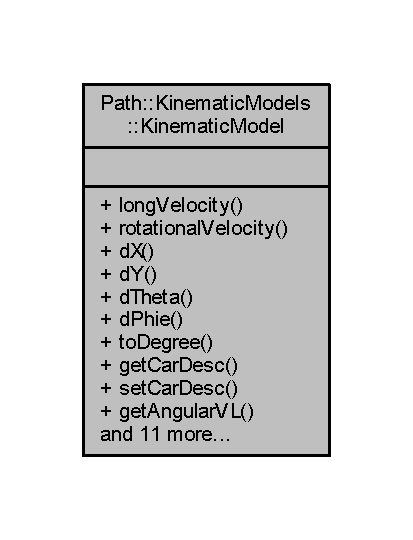
\includegraphics[width=198pt]{d1/d1c/class_path_1_1_kinematic_models_1_1_kinematic_model__coll__graph}
\end{center}
\end{figure}
\subsection*{Public Member Functions}
\begin{DoxyCompactItemize}
\item 
\mbox{\Hypertarget{class_path_1_1_kinematic_models_1_1_kinematic_model_aaa589d746eae3d1f4fe104308c2e6326}\label{class_path_1_1_kinematic_models_1_1_kinematic_model_aaa589d746eae3d1f4fe104308c2e6326}} 
virtual double {\bfseries long\+Velocity} () const
\item 
\mbox{\Hypertarget{class_path_1_1_kinematic_models_1_1_kinematic_model_a2fe4e8e6a4ce76a9454c8d1ff148e0b9}\label{class_path_1_1_kinematic_models_1_1_kinematic_model_a2fe4e8e6a4ce76a9454c8d1ff148e0b9}} 
virtual double {\bfseries rotational\+Velocity} () const
\item 
\mbox{\Hypertarget{class_path_1_1_kinematic_models_1_1_kinematic_model_a60745cb4bc8afea4c95980d3057a66b1}\label{class_path_1_1_kinematic_models_1_1_kinematic_model_a60745cb4bc8afea4c95980d3057a66b1}} 
virtual double {\bfseries dX} () const
\item 
\mbox{\Hypertarget{class_path_1_1_kinematic_models_1_1_kinematic_model_adc7234f8230ff513807a3c21f1bd6d10}\label{class_path_1_1_kinematic_models_1_1_kinematic_model_adc7234f8230ff513807a3c21f1bd6d10}} 
virtual double {\bfseries dY} () const
\item 
\mbox{\Hypertarget{class_path_1_1_kinematic_models_1_1_kinematic_model_aeb5bd3e94024cc3844df7e6affea8284}\label{class_path_1_1_kinematic_models_1_1_kinematic_model_aeb5bd3e94024cc3844df7e6affea8284}} 
virtual double {\bfseries d\+Theta} () const
\item 
\mbox{\Hypertarget{class_path_1_1_kinematic_models_1_1_kinematic_model_a5a36a55326a1b3c4e5ead7d9d14b9971}\label{class_path_1_1_kinematic_models_1_1_kinematic_model_a5a36a55326a1b3c4e5ead7d9d14b9971}} 
virtual double {\bfseries d\+Phie} () const
\item 
\mbox{\Hypertarget{class_path_1_1_kinematic_models_1_1_kinematic_model_aaa6e2e81a1c72af570307a363b513f62}\label{class_path_1_1_kinematic_models_1_1_kinematic_model_aaa6e2e81a1c72af570307a363b513f62}} 
virtual double {\bfseries to\+Degree} (const double \&rad) const
\item 
\mbox{\Hypertarget{class_path_1_1_kinematic_models_1_1_kinematic_model_a67d1a31ddc271fda6637c3d0f48e6929}\label{class_path_1_1_kinematic_models_1_1_kinematic_model_a67d1a31ddc271fda6637c3d0f48e6929}} 
\hyperlink{class_path_1_1_kinematic_models_1_1_car_description}{Car\+Description} $\ast$ {\bfseries get\+Car\+Desc} () const
\item 
\mbox{\Hypertarget{class_path_1_1_kinematic_models_1_1_kinematic_model_a340bc6ab51ba9841e7745f337c0351a7}\label{class_path_1_1_kinematic_models_1_1_kinematic_model_a340bc6ab51ba9841e7745f337c0351a7}} 
void {\bfseries set\+Car\+Desc} (\hyperlink{class_path_1_1_kinematic_models_1_1_car_description}{Car\+Description} $\ast$value)
\item 
\mbox{\Hypertarget{class_path_1_1_kinematic_models_1_1_kinematic_model_a41a20b17d27788184b57df21c6c43b72}\label{class_path_1_1_kinematic_models_1_1_kinematic_model_a41a20b17d27788184b57df21c6c43b72}} 
double {\bfseries get\+Angular\+VL} () const
\item 
\mbox{\Hypertarget{class_path_1_1_kinematic_models_1_1_kinematic_model_a0232dd0559ee9de4fa1bde032053c4fb}\label{class_path_1_1_kinematic_models_1_1_kinematic_model_a0232dd0559ee9de4fa1bde032053c4fb}} 
void {\bfseries set\+Angular\+VL} (double value)
\item 
\mbox{\Hypertarget{class_path_1_1_kinematic_models_1_1_kinematic_model_a7a1d16fd771907c8fad093ad73fe966d}\label{class_path_1_1_kinematic_models_1_1_kinematic_model_a7a1d16fd771907c8fad093ad73fe966d}} 
double {\bfseries get\+Angular\+VR} () const
\item 
\mbox{\Hypertarget{class_path_1_1_kinematic_models_1_1_kinematic_model_a8ae837f60257f543bb8fe1371f3c6238}\label{class_path_1_1_kinematic_models_1_1_kinematic_model_a8ae837f60257f543bb8fe1371f3c6238}} 
void {\bfseries set\+Angular\+VR} (double value)
\item 
\mbox{\Hypertarget{class_path_1_1_kinematic_models_1_1_kinematic_model_a5c771a657e0d70480361ad0b81b2ff8c}\label{class_path_1_1_kinematic_models_1_1_kinematic_model_a5c771a657e0d70480361ad0b81b2ff8c}} 
double {\bfseries get\+Theta} () const
\item 
\mbox{\Hypertarget{class_path_1_1_kinematic_models_1_1_kinematic_model_a155899b508df1f386de1174a7cb33e5f}\label{class_path_1_1_kinematic_models_1_1_kinematic_model_a155899b508df1f386de1174a7cb33e5f}} 
void {\bfseries set\+Theta} (double value)
\item 
\mbox{\Hypertarget{class_path_1_1_kinematic_models_1_1_kinematic_model_a01bdc3a2b497e16238db243539e5b0dc}\label{class_path_1_1_kinematic_models_1_1_kinematic_model_a01bdc3a2b497e16238db243539e5b0dc}} 
double {\bfseries get\+U1} () const
\item 
\mbox{\Hypertarget{class_path_1_1_kinematic_models_1_1_kinematic_model_a49e08a8f9579da776d922973cc129d92}\label{class_path_1_1_kinematic_models_1_1_kinematic_model_a49e08a8f9579da776d922973cc129d92}} 
void {\bfseries set\+U1} (double value)
\item 
\mbox{\Hypertarget{class_path_1_1_kinematic_models_1_1_kinematic_model_a4d41edca86841bbace00ae577dc8f524}\label{class_path_1_1_kinematic_models_1_1_kinematic_model_a4d41edca86841bbace00ae577dc8f524}} 
double {\bfseries get\+U2} () const
\item 
\mbox{\Hypertarget{class_path_1_1_kinematic_models_1_1_kinematic_model_a1be6902520ab6ae8ac53fd98344e7cc9}\label{class_path_1_1_kinematic_models_1_1_kinematic_model_a1be6902520ab6ae8ac53fd98344e7cc9}} 
void {\bfseries set\+U2} (double value)
\item 
\mbox{\Hypertarget{class_path_1_1_kinematic_models_1_1_kinematic_model_aa00779de34c5c6fe2d3b1ef91544ff09}\label{class_path_1_1_kinematic_models_1_1_kinematic_model_aa00779de34c5c6fe2d3b1ef91544ff09}} 
double {\bfseries get\+Phie} () const
\item 
\mbox{\Hypertarget{class_path_1_1_kinematic_models_1_1_kinematic_model_a900c3ce6d136bc414893d486bb4480b9}\label{class_path_1_1_kinematic_models_1_1_kinematic_model_a900c3ce6d136bc414893d486bb4480b9}} 
void {\bfseries set\+Phie} (double value)
\end{DoxyCompactItemize}


The documentation for this class was generated from the following files\+:\begin{DoxyCompactItemize}
\item 
Car\+Model/\+Car\+Model\+Qt/\+Car\+Math\+Model/\+Path\+Tracking/basekinematicmodel/kinematicmodel.\+h\item 
Car\+Model/\+Car\+Model\+Qt/\+Car\+Math\+Model/\+Path\+Tracking/basekinematicmodel/kinematicmodel.\+cpp\end{DoxyCompactItemize}

%--- End generated contents ---

% Index
\backmatter
\newpage
\phantomsection
\clearemptydoublepage
\addcontentsline{toc}{chapter}{Index}
\printindex

\end{document}
